\section{Summary}

A selection designed to be uniformly efficient in all regions of the dark boson's mass-lifetime
parameter space has been presented with a view to embarking on a search for a new dark boson.
A frequentist method designed to search for an signal in any arbitrary mass spectrum has also been
presented and used in the case of the dimuon mass spectrum from \btokstrmumu.

This strategy has extracted a $p$-value of a particle considering test masses which do not go all
the way to the boundaries of various vetoes in the invariant dimuon mass spectrum.
It is determined that the maximum deviation of the selected candidates from the null hypothesis of
zero signal has a global significance of $0.63\stdev$ at $m_t = 4285.0\mev$.
This is consistent with no new particle in the \mumu distribution over the mass ranges probed.
The full analysis will get much closer to these edges and probe the interesting $m_{\mumu}=214\mev$
region.
The next step in the analysis is to set limits and present them in a model independent way.
Of course, they can be translated to specific models for interpretation.

%Figure~\ref{fig:db:excl} shows projected exclusion regions from this analysis.
%Figure~\ref{fig:db:excl:inf} shows projected exclusion regions for the inflaton
%model~\cite{Bezrukov:2014nza}, and axion model~\cite{Freytsis:2009ct}.


\subsection{The official LHCb analysis}
\added{
The entire analysis described in this chapter, including strategy and selection, was completed
as part of the official \lhcb analysis after this thesis was submitted, and therefore results to
include in this thesis were calculated separately, as given above.
Since then the \lhcb analysis has been published in Ref.~\cite{LHCb-PAPER-2015-036}.
There are a few differences between the two analysis.
Firstly the \lhcb analysis covered the entire range in $m_{\mumu}$, going very close to the
kinematic boundaries.
The conversion of local to global $p$-value was made using a \PDF constructed from cubic spline
interpolation and generating toys in bins, rather than continuously.
Finally, the decision was made in the \lhcb analysis to veto the region around the $\omega$ mass,
because the branching fraction $\BF\big(\Bd\!\to\Kstarz\omega(\to\mumu)\big)$ is relatively large
(as shown in \Tab{tab:db:bkg}) and therefore there is some chance of observing interference
effects.
The \phii and $\omega$ vetoes also only apply in the prompt regions.
The minimum local excess in the official \lhcb analysis appears at $\mass{\db}=253\mev$ with a
$p$-value of about 0.8, consistent with no new physics.
This is just outside the range of the results given above.
The published plane of upper limits for $\BF\big(\Bd\!\to\Kstarz\db(\mumu)\big) /
\BF\big(\btokstrmumu\big)_{[1.1,6.0]\gevgev}$ and $\BF\big(\Bd\!\to\Kstarz\db(\mumu)\big)$ at
$95\pc$ CL are shown in \Fig{fig:db:excl:infl}.
These limits take into account the systematic uncertainties from the previous section.
A model dependent exclusion region for the inflaton is shown in Fig.~\ref{fig:db:excl:infl:model}.
}


%\deleted{
%Figure~\ref{fig:db:excl:infl} shows the projected
%sensitivity of this analysis to the inflaton model in Ref.~\cite{Bezrukov:2014nza}.
%There is a region excluded by theory, where the model does not satisfy known cosmological
%constraints.
%It is predicted that it should be possible to rule out the mass range
%$250<\mass{\db}<450\mev$ entirely, and come within an order of magnitude of mixing parameter
%$\theta^2$ for masses up to $1000\mev$.
%Assumptions made in making this are that: the lifetime of the inflaton is in the range
%$1<\lifetime{\db}<1000\ps$, that $\BF(\btokstrdb)\simeq10^{-6}$,
%and that the \db has the same couplings as the Higgs boson.
%}
%%and that $\BF(\dbtomumu)$
%is the same for a Higgs boson with the mass of an inflaton.

\begin{figure}
  \begin{center}
    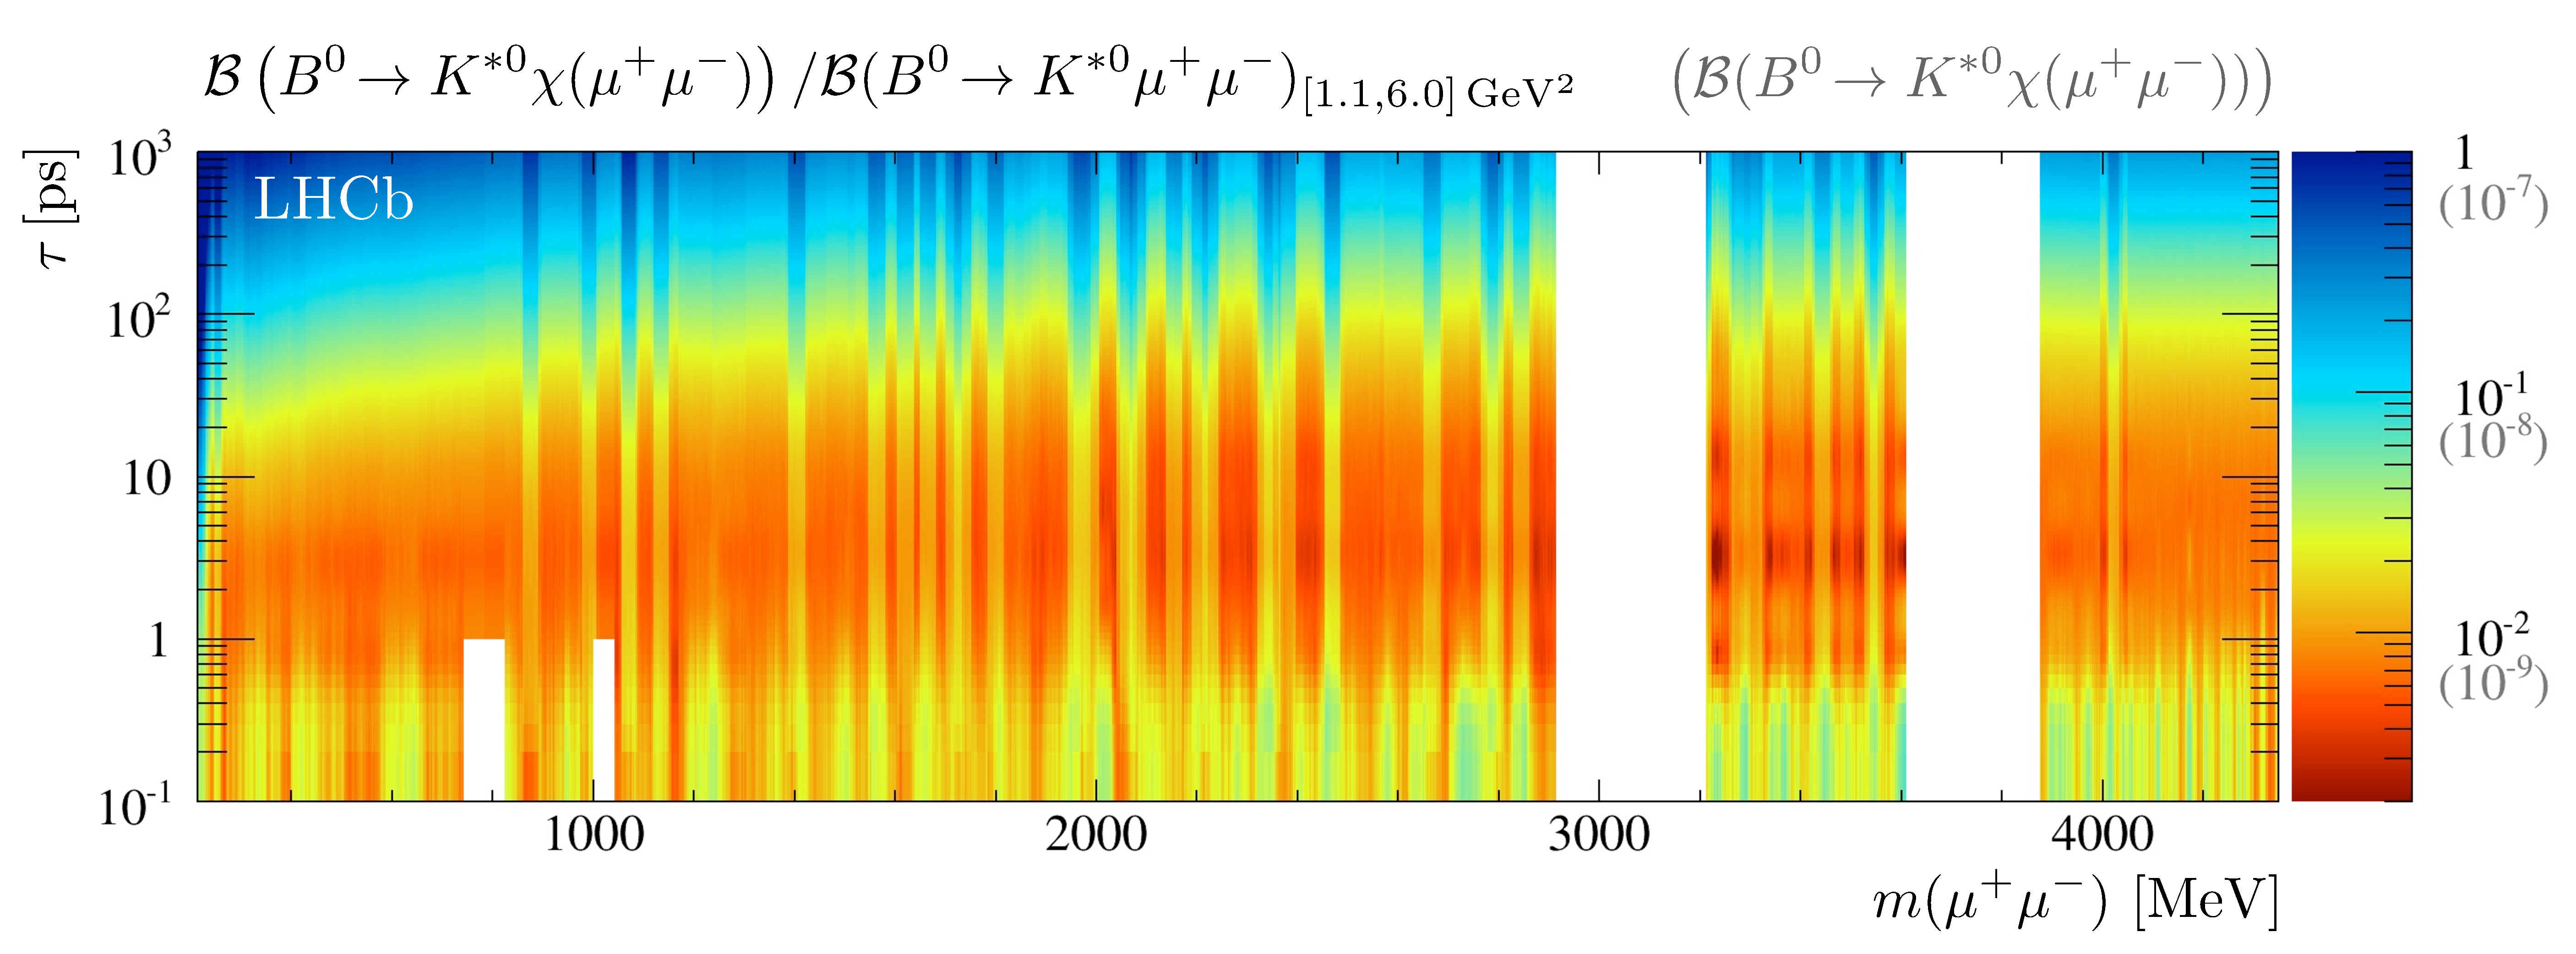
\includegraphics[width=\textwidth]{axion_lims}
    \caption[Projected sensitivity in an inflaton search]
    {
      Upper limits for
      $\BF\big(\Bd\!\to\Kstarz\db(\mumu)\big) / \BF\big(\btokstrmumu\big)_{[1.1,6.0]\gevgev}$
      and $\BF\big(\Bd\!\to\Kstarz\db(\mumu)\big)$ at $95\pc$ CL.
      Vetoed regions for the \jpsi and \psitwos can be seen for all lifetime regions, while the
      $\omega$ and $\phi$ regions are removed in only the prompt region.
      This figure is taken from Ref.~\protect\cite{LHCb-PAPER-2015-036}.
    }
    \label{fig:db:excl:infl}
  \end{center}
\end{figure}


\begin{figure}
  \begin{center}
    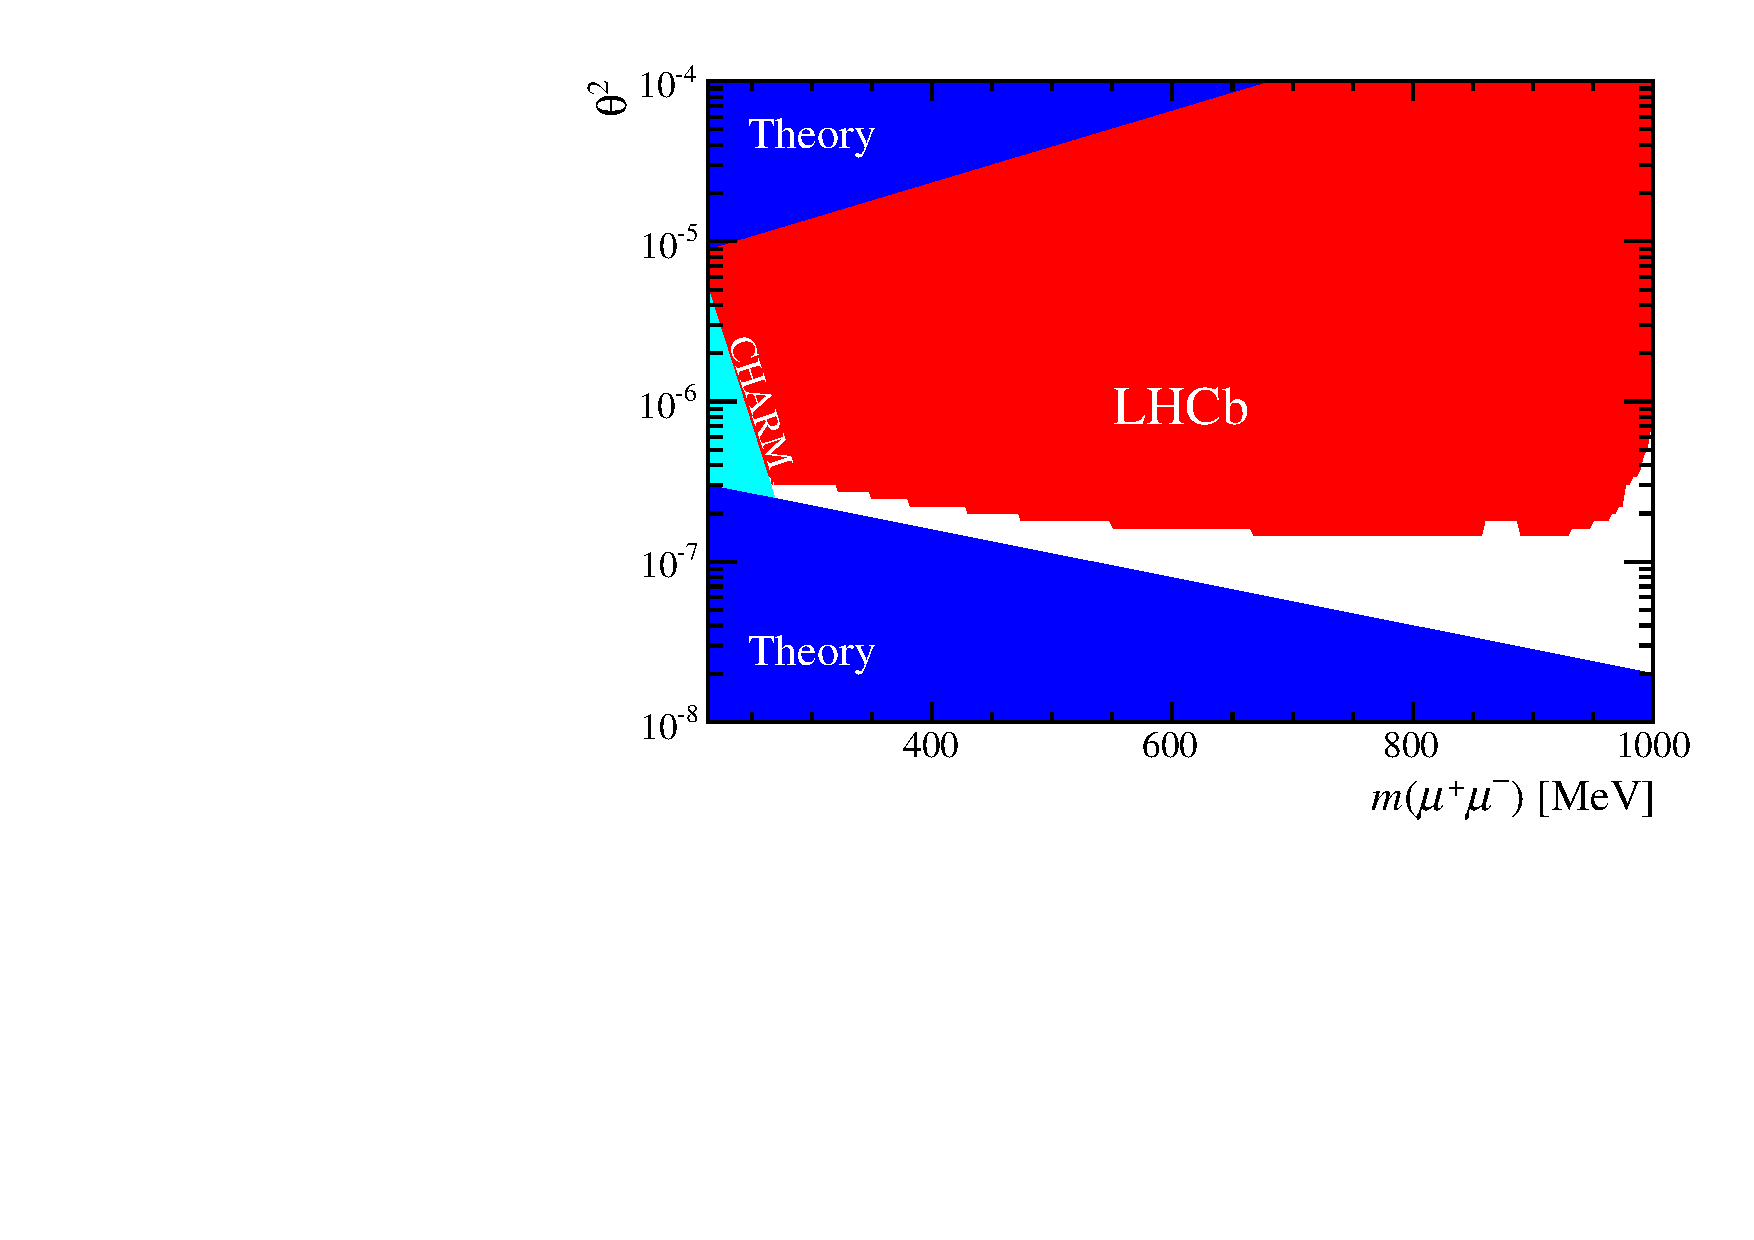
\includegraphics[width=0.65\textwidth]{kstmm_infl_excl}
    \caption[Projected sensitivity in an inflaton search]
    {
      Projected exclusion regions for an inflaton model from Ref.~\protect\cite{Bezrukov:2014nza},
      in the mass range $1<\mass{\db}<1000\mev$ to $95\%$ CL, this region and model is the same as
      the plane in
      parameter space shown in Fig.~\protect\ref{fig:db:inflaton}.
      The region below the red line is excluded by theory, since the model fails cosmological
      constraints in this region.
      In this mass range, it is expected that this analysis will exclude all but a small area of
      parameter space for this model.
    }
    \label{fig:db:excl:infl:model}
  \end{center}
\end{figure}






